
\section{DVS Implementation}
DVS (Dynamic Vision Sensor) is a newly developed instruments for vision data acquisition which imitates the function of human eyes. In this section, we first introduce the DVS theory which we will apply and then modify the data-set into "fake" DVS data-set, which means that we generate  data-set to imitate the DVS-like data-set. Finally we will use these data set to train our fcn network, which is already discussed in \emph{Section \Romannum{3}} .

\subsection{DVS theory}

\begin{figure}
	\centering\textbf{}
	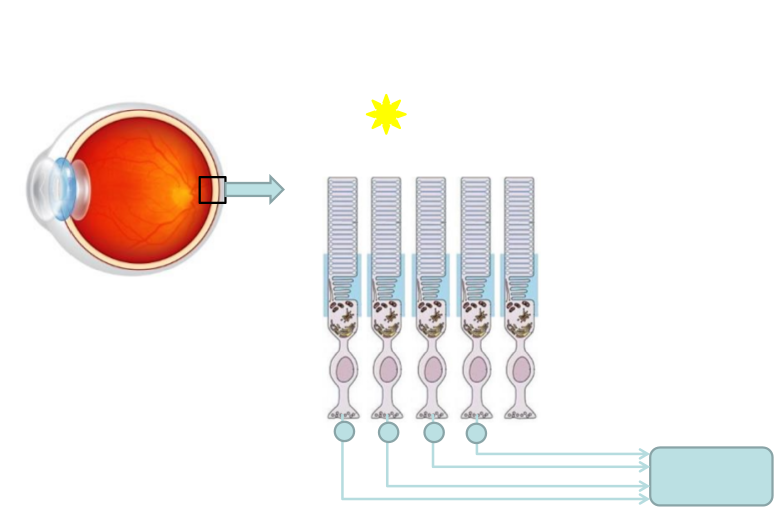
\includegraphics[width=0.4\textwidth]{human_vision.png}
	\caption{Human Vision System\cite{davide}}
	\label{fig:humanvision}
\end{figure}

Nowadays, we are used to record a scene by taking a picture or video. Frame-base devices are dominant in daily life. It is natural that we record a piece of event by filming them frame by frame no matter what devices we use, like CCD or CMOS. The advantages are obvious, they have small simole pixels, leading to high resolution, large fill factor and low imager cost. The output format is understandable and this is the basis for many years of research in computer vision. However, frame-base architecture has high cost when storing information where the intensity of pixels never change based on a series of snapshots taken at a constant rate. The latency of the vision requires high-speed frame rate, which results massive output-data. \cite{lichtsteiner2008128}. The basic problem of frame-based architecure is the hight latency and temporal discretization. The average latency of robot vision algorithm is about 50-200ms, which constrains the development of robotics in high-speed scenarios, such as autonomous driving or unmanned aerial vehicle.

Inspired by human vision system, seen in Figure \ref{fig:humanvision}, the retinal outputs are massively parallel and data driven. The neurons of the retina do not spike all at the same time. In vertebrates, the decisions on when to quantize are made by the ganglion cells that project to the brain and that send their information in the form of digital events which occur in continuous time.\cite{liu2015event} 

Therefore, dynamic vision sensor (DVS) is designed to meet the challenge of the processing speed with traditional on-board cameras. DVS outputs asynchronous evens at microsecond resolution, while traditional camera outputs frames frames at fixed time intervals. An event is generated each time a single pixel changes value. If the change in brightness is larger than \emph{C} then, an \emph{on event} will be generated, if smaller than \emph{-C}, \emph{off event} will be produced, seen in Figure \ref{fig:dvsscheme}. However, these DVS generated "pictures" are quite different from common-used pictures, which is based on the frame. To integrate DVS into training FCN, there is still a lot of work to to in data reprocessing. By accumulate all events occurred in a time interval $\Delta t$, we can visualize the event stream. Such as we accumulate all events of a rotating dot in a time interval, then in visualization, it could be a circle. When the time increases, the brightness of this circle will be darker. Based on that simple rule, we can thus in next section to produce a "fake" DVS data-base using common dataset used to train ConvNets.
\begin{figure}
	\centering\textbf{}
	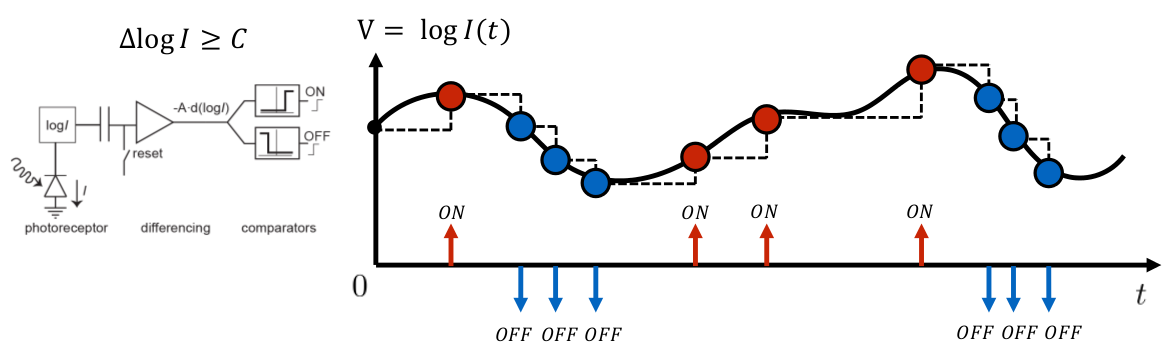
\includegraphics[width=0.5\textwidth]{dvsschem.png}
	\caption{DVS Operation Principle\cite{davide}}
	\label{fig:dvsscheme}
\end{figure}

\subsection{DVS Dataset}

\begin{figure}
\centering
\subfigure[DVS Image with clutter]{
\begin{minipage}[b]{0.2\textwidth}
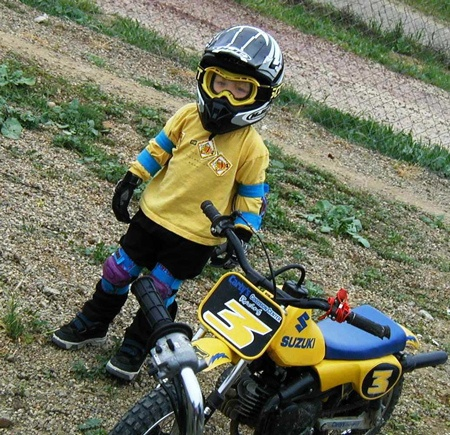
\includegraphics[width=0.9\textwidth]{1.jpg} \\
\label{fig:withclutter}
\\
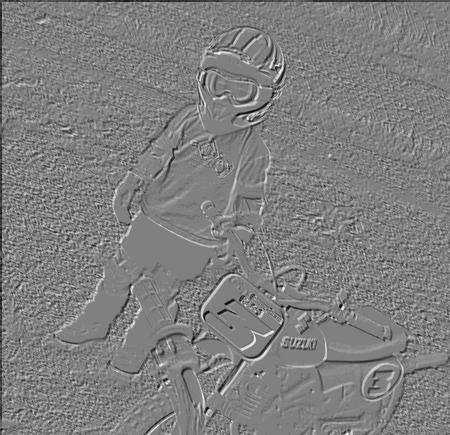
\includegraphics[width=0.9\textwidth]{1_DVS.jpg}
\end{minipage}
}
\subfigure[DVS Image without clutter]{
\begin{minipage}[b]{0.2\textwidth}
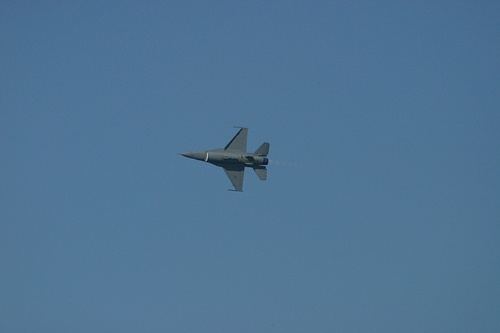
\includegraphics[width=1.2\textwidth]{2.jpg} 
\label{fig:withoutclutter}\\
\\
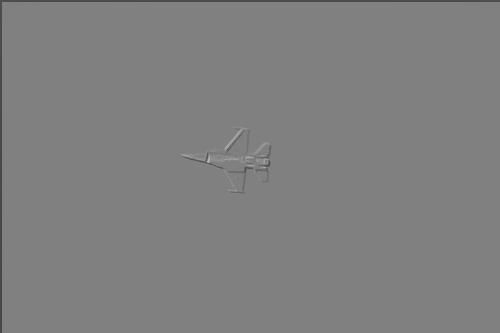
\includegraphics[width=1.2\textwidth]{2_DVS.jpg}
\end{minipage}
}
\caption{DVS Data Set}
\label{fig:dvsdata}
\end{figure}

Here we transfer data set consisted of over 10000 pictures from +++++ into fake event base data set, seen in Figure \ref{fig:dvsdata}. We first scale the images into gray images A. Then shift each image to a random direction to produce an "event" in image B. It imitates the motion of an object in the picture. Next, we subtract the gray scaled image A with shifted image B, which results a change over pixels. We produce "events" by means of assuming a threshold $C$. If the change of pixel intensity is larger than $C$, then it is an \emph{on event}. On the  contrary, if the change of pixel intensity is the smaller than $-C$, then is is an \emph{off event}. Within the interval $[-C,C]$, there exits no event. The Equations are derived as follows
\begin{equation}
    I_{i,j}^{new} =
    \begin{cases}
    \frac{\Delta I_{i,j}}{2(1-C)}+\frac{1}{2(1-C)} &\mbox{$\Delta I_{i,j}\in [-1,-C]$ \emph{off event}}\\
    \frac{1}{2} &\mbox{$\Delta I_{i,j}\in [-C,C]$ \,\emph{no event}}\\
    \frac{\Delta I_{i,j}}{2(1-C)}+\frac{1-2C}{2(1-C)} &\mbox{$\Delta I_{i,j}\in [C,1]$\,\,\,\,\,\emph{on event}}
   \end{cases}
  \end{equation}
where $I_{i,j}^{new}$ is the resulting intensity of the corresponding pixel $(i,j)$, $\Delta I_{i,j}$ is the difference of intensity of the same pixel $(i,j)$ from image A and image B. Note that, in programme, we scale the intensity interval into $[0,1]$.

However, this procedure will make every single thing in the picture moving in a certain direction. If the scene we take has no so much clutter, the result images is quite smoothing, on contrast, if the scene has so much clutter like Image \ref{fig:withclutter}, then the resulting image will be filled by "events". Thus, DVS data can not deal with the scene with much clutter, because it can not give us "useful " information about the object. However, like the Figure \ref{fig:withoutclutter}, the outline of the object "airplane" is obvious. If we use real DVS data, it can be clearly inferred that the direction of the flight without any other redundancy

\subsection{Training based on DVS data set}
After generating the data-set we use in FCN network previously, we can now train the network based on the DVS data set. During training, we find that the loss function can not converge. Seen in Figure.

% \begin{figure*}
%     \centering
%     \subfigure{
%     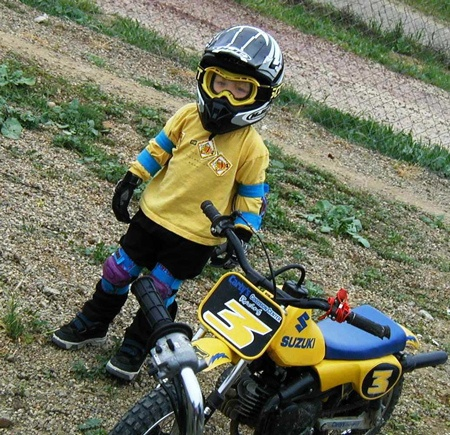
\includegraphics[width=0.25\textwidth]{1.jpg}
%     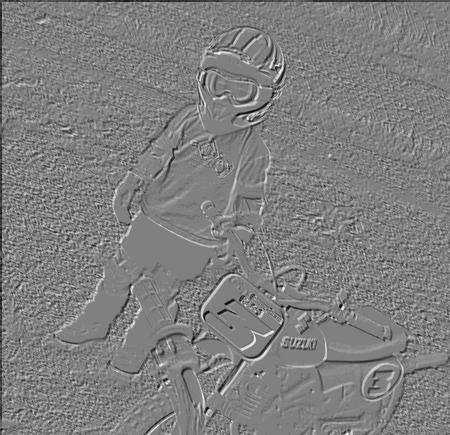
\includegraphics[width=0.25\textwidth]{1_DVS.jpg}
%     \caption{DVS with clusters}
%     }
    
%     \subfigure{
    
%     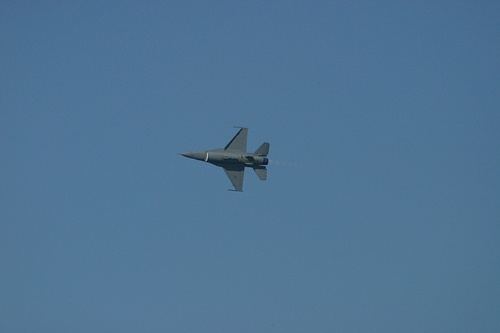
\includegraphics[width=0.3\textwidth]{2.jpg}
%     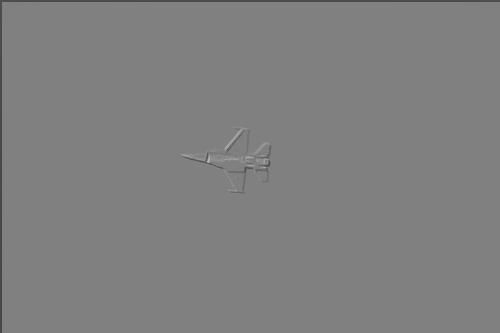
\includegraphics[width=0.3\textwidth]{2_DVS.jpg}
%     \caption{DVS without clusters}
%     }
% \end{figure*}

%\begin{figure}
%	\centering
%	\includegraphics[width=0.4\textwidth]{}
%\end{figure}
